\documentclass[11pt,fleqn]{article}

\usepackage{latexsym}
\usepackage{makeidx}
\usepackage{url}
\usepackage{xspace}
\usepackage{graphicx}

\input{version}

%%% ------------------------------------------------------------------

\usepackage[colorlinks,linkcolor=blue]{hyperref}
\hypersetup{bookmarksopen=true}
\hypersetup{bookmarksopenlevel=0}
\hypersetup{pdftitle={KiCS2: The Kiel Curry System Version 2}}
\hypersetup{pdfauthor={Michael Hanus}}
%\hypersetup{pdfstartview=Title}
\hypersetup{pdfstartview=FitH}
\usepackage{thumbpdf}

%%% ------------------------------------------------------------------

\setlength{\textwidth}{16.5cm}
\setlength{\textheight}{23cm}
\renewcommand{\baselinestretch}{1.1}
\setlength{\topmargin}{-1cm}
\setlength{\oddsidemargin}{0cm}
\setlength{\evensidemargin}{0cm}
\setlength{\marginparwidth}{0.0cm}
\setlength{\marginparsep}{0.0cm}

\newlength{\figurewidth}
\setlength{\figurewidth}{\textwidth}
\addtolength{\figurewidth}{-0.4cm}

% font for program texts
\renewcommand{\tt}{\usefont{OT1}{cmtt}{m}{n}\selectfont}
\newcommand{\codefont}{\small\tt}

\usepackage{listings}
\lstset{aboveskip=1.5ex,
        belowskip=1.5ex,
        showstringspaces=false, % no special string space
        mathescape=true,
        flexiblecolumns=false,
        xleftmargin=2ex,
        basewidth=0.52em,
        basicstyle=\small\ttfamily}

\lstset{literate={->}{{$\rightarrow{}\!\!\!$}}3
       }

\lstnewenvironment{curry}{}{}
\newcommand{\listline}{\vrule width0pt depth1.75ex}

% program text in normal text
\newcommand{\code}[1]{\mbox{\codefont #1}}

% program text in normal text with apostrophs
\newcommand{\ccode}[1]{``\code{#1}''}

\newcommand{\pindex}[1]{\index{#1@{\tt #1}}}  % program elements in index

\newcommand{\labs}{\mbox{\tt\char92}}  % lambda abstraction in Curry
\newcommand{\todo}[1]{\fbox{\sc To do: #1}}
\newcommand{\cb}{CurryBrowser\xspace}

% allow underscores in programs:
\catcode`\_=\active
\let_=\sb
\catcode`\_=12

% produce an index:
\makeindex

\begin{document}
\sloppy

\begin{titlepage}
\pdfbookmark[1]{Title}{Title}
\begin{center}
\fbox{
\begin{minipage}[t]{\figurewidth}
\begin{center}\vspace{10ex}
{\Huge\bf KiCS2}\\[4ex]
{\huge The Kiel Curry System (Version 2)}\\[7ex]
{\huge User Manual}\\[4ex]
\kicsversiondate\\[6ex]
\Large
Michael Hanus$^1$ [editor] \\[3ex]
{\large Additional Contributors:}\\[2ex]
Bernd Bra\ss{}el$^2$ \\
Bj\"orn Peem\"oller$^3$\\
Fabian Reck$^4$ \\[4ex]
\normalsize
(1) University of Kiel, Germany, {\tt mh@informatik.uni-kiel.de} \\
(2) University of Kiel, Germany, {\tt bbr@informatik.uni-kiel.de} \\
(3) University of Kiel, Germany, {\tt bjp@informatik.uni-kiel.de} \\
(4) University of Kiel, Germany, {\tt fre@informatik.uni-kiel.de} \\[5ex]~
\end{center}
\end{minipage}}
\end{center}
\end{titlepage}

\pdfbookmark[1]{Contents}{Contents}
\tableofcontents

\newpage

\addcontentsline{toc}{section}{Preface}
\section*{Preface}

This document describes KiCS2 (\textbf{Ki}el \textbf{C}urry \textbf{S}ystem
Version \textbf{2}),
an implementation of the multi-paradigm language Curry
\cite{Hanus97POPL,Hanus06Curry} that is
based on compiling Curry programs into Haskell programs.
Curry is a universal programming language aiming at the amalgamation
of the most important declarative programming paradigms,
namely functional programming and logic programming.  
Curry combines in a seamless way features from functional programming
(nested expressions, lazy evaluation, higher-order functions),
logic programming (logical variables, partial data structures,
built-in search), and concurrent programming (concurrent evaluation
of constraints with synchronization on logical variables).
The current KiCS2 implementation does not support concurrent
constraints. Alternatively, one can write distributed applications
by the use of sockets that can be registered and accessed
with symbolic names.
Moreover, KiCS2 also supports
the high-level implementation of
graphical user interfaces and web services
(as described in more detail in
\cite{Hanus99PPDP,Hanus00PADL,Hanus01PADL,Hanus06PPDP}).

We assume familiarity with the ideas and features
of Curry as described in the Curry language definition \cite{Hanus12Curry}.
Therefore, this document only explains the use of the different
components of KiCS2
and the differences and restrictions of KiCS2
(see Section~\ref{sec-restrictions})
compared with the language Curry (Version 0.8.3).
The basic ideas of the implementation of KiCS2
can be found in
\cite{BrasselHanusPeemoellerReck11,BrasselHanusPeemoellerReck11WLP}.

\bigskip

\subsection*{Acknowledgements}

This work has been supported in part by the
DFG grants Ha 2457/5-1 and Ha 2457/5-2.

\newpage

\section{Overview of KiCS2}

\subsection{Installation}
\label{sec-install}

This version of KiCS2 has been developed and
tested on Linux systems.
In principle, it should be also executable on other
platforms on which a Haskell implementation (Glasgow Haskell Compiler
and Cabal) exists, like in many Linux distributions, Sun Solaris,
or Mac OS X systems.

Installation instructions for KiCS2 can be found in
the file \code{INSTALL.txt} stored in the KiCS2 installation directory.
Note that there are two possibilities to install KiCS2:
\begin{description}
\item[Global installation:]\index{global installation}\index{installation!global}
KiCS2 is installed in some global system directory where users
have no write permission. In this case, some options for experimenting
with KiCS2 (like \code{supply} or \code{ghc}, see below)
are not available (since they require the recompilation of parts of
the installed system).
\item[Local installation:]\index{local installation}\index{installation!local}
KiCS2 is installed in some local user directory where the user
has write permission and the option \code{GLOBALINSTALL}
in the \code{Makefile} of the KiCS2 installation is set as follows:
\begin{lstlisting}
GLOBALINSTALL=no
\end{lstlisting}
In this case, all options of KiCS2 are available.
\end{description}
In the following, $kics2home$ denotes the installation directory
of the KiCS2 installation.


\subsection{General Use}
\label{sec-general}

All executables required to use the different components
of KiCS2 are stored in the directory \code{$kics2home$/bin}.
You should add this directory
to your path (e.g., by the \code{bash} command
\ccode{export PATH=$kics2home$/bin:\$PATH}).

The source code of the Curry program
must be stored in a file with the suffix \ccode{.curry},
e.g., \code{prog.curry}. 
Literate programs must be stored in files with the extension \ccode{.lcurry}.

Since the translation of Curry programs with KiCS2 creates
some auxiliary files (see Section~\ref{sec-auxfiles} for details),
you need write permission
in the directory where you have stored your Curry programs.
Moreover, the current implementation also recompiles
system libraries according to the setting of some options.
Therefore, the KiCS2 system should be locally installed
in your user account.
The auxiliary files for all Curry programs in the current
directory can be deleted by the command\pindex{cleancurry}
\begin{curry}
cleancurry
\end{curry}
(this is a shell script stored in the \code{bin} directory of the
KiCS2 installation, see above).
The command
\begin{curry}
cleancurry -r
\end{curry}
also deletes the auxiliary files in all subdirectories.



\subsection{Restrictions}
\label{sec-restrictions}

There are a few minor restrictions on Curry programs
when they are processed with KiCS2:
\begin{itemize}
\item
\index{singleton variables}\index{variables!singleton}
\emph{Singleton pattern variables}, i.e., variables that occur only once
in a rule, should be denoted as an anonymous variable \ccode{_},
otherwise the parser will print a warning since this is a
typical source of programming errors.
\item
KiCS2 translates all \emph{local declarations} into global functions with
additional arguments (``lambda lifting'', see Appendix~D of the
Curry language report).
Thus, in the various run-time systems, the definition of
functions with local declarations look different from
their original definition (in order to see the result
of this transformation, you can use the \cb, see
Section~\ref{sec-currybrowser}).
\item \index{tabulator stops}
Tabulator stops instead of blank spaces in source files are
interpreted as stops at columns 9, 17, 25, 33, and so on.
In general, tabulator stops should be avoided in source programs.
\item
Encapsulated search\index{encapsulated search}: In order
to allow the integration of non-deterministic computations
in programs performing I/O at the top-level, KiCS2 provides
the libraries \code{AllSolutions} (Section~\ref{Library:AllSolutions})
and \code{SearchTree} (Section~\ref{Library:SearchTree})
where one can defined search operators and various search strategies.
The general definition of encapsulated search of the Curry report
\cite{HanusSteiner98PLILP} is not supported.
\item Concurrent computations\index{concurrency}
based on the suspension of expressions
containing free variables are not yet supported.
KiCS2 supports \emph{value generators} for free variables
so that a free variable is instantiated when its value is demanded.
For instance, the initial expression
\begin{curry}
x == True where x free
\end{curry}
is non-deterministically evaluated to \code{False} and \code{True}
by instantiating \code{x} to \code{False} and \code{True}, respectively.
Thus, a computation is never suspended due to free variables.
This behavior also applies to free variables of primitive types
like integers. For instance, the initial expression
\begin{curry}
x*y=:=1 where x,y free
\end{curry}
is non-deterministically evaluated to the two solutions
\begin{curry}
{x = -1, y = -1} Success
{x = 1, y = 1} Success
\end{curry}
\item
Unification is performed without an occur check.
\item
There is currently no general connection to external constraint solvers.
\end{itemize}


\subsection{Modules in KiCS2}
\label{sec-modules}

The current implementation of KiCS2 supports only flat module names,
i.e., the notation \code{Dir.Mod.f} is not supported.\index{modules}
In order to allow the structuring of modules in different directories,
KiCS2 searches for imported modules in various directories.
By default, imported modules are searched in the directory
of the main program and the system module directories
\ccode{$kics2home$/lib} and \ccode{$kics2home$/lib/meta}.
This search path can be extended
by setting the environment variable \code{CURRYPATH}\pindex{CURRYPATH}
(which can be also set in a KiCS2 session by the option
\ccode{:set path}\pindex{path}\pindex{:set path},
see below)
to a list of directory names separated by colons (\ccode{:}).
In addition, a local standard search path
can be defined in the \ccode{.kics2rc} file
(see Section~\ref{sec-customization}).
Thus, modules to be loaded are searched in the following
directories (in this order, i.e., the first occurrence of a module file
in this search path is imported):
\begin{enumerate}
\item Current working directory (\ccode{.}) or directory prefix
of the main module (e.g., directory \ccode{/home/joe/curryprogs}
if one loads the Curry program \ccode{/home/joe/curryprogs/main}).
\item The directories enumerated in the environment variable \code{CURRYPATH}.
\item The directories enumerated in the \ccode{.kics2rc} variable
      \ccode{libraries}.
\item The directories \ccode{$kics2home$/lib} and \ccode{$kics2home$/lib/meta}.
\end{enumerate}
Note that the standard prelude (\code{$kics2home$/lib/Prelude.curry})
will be always implicitly imported to all modules if a module
does not contain an explicit import declaration for the module
\code{Prelude}.


\newpage

\section{Using the Interactive Environment of KiCS2}
\label{sec-kics2}

This section describes the interactive environment
KiCS2\index{KiCS2}
that supports the development of applications written in Curry.
The implementation of KiCS2 contains also a separate compiler
which is automatically invoked by the interactive environment.

\subsection{Invoking KiCS2}
\label{sec:invoke-kics2}

To start KiCS2, execute the command
\ccode{kics2}\pindex{kics2}
(this is a shell script stored in
\code{$kics2home$/bin} where $kics2home$ is the installation directory
of KiCS2).
When the system is ready (i.e., when the prompt \ccode{Prelude>} occurs),
the prelude (\code{$kics2home$/lib/Prelude.curry})
is already loaded, i.e., all definitions in the prelude are accessible.
Now you can type various commands (see next section)
or an expression to be evaluated.

One can also invoke KiCS2 with parameters.
These parameters are usual a sequence of commands
(see next section) that are executed before the user interaction
starts. For instance, the invocation
\begin{curry}
kics2 :load Mod :add List
\end{curry}
starts KiCS2, loads the main module \code{Mod}, and adds the additional
module \code{List}.
The invocation
\begin{curry}
kics2 :load Mod :eval config
\end{curry}
starts KiCS2, loads the main module \code{Mod}, and evaluates
the operation \code{config} before the user interaction starts.
As a final example, the invocation
\begin{curry}
kics2 :load Mod :save :quit
\end{curry}
starts KiCS2, loads the main module \code{Mod}, creates an executable,
and terminates KiCS2. This invocation could be useful in ``make'' files
for systems implemented in Curry.


\subsection{Command of KiCS2}
\label{sec:kics2-commands}

The {\bf most important commands} of KiCS2 are
(it is sufficient to type a unique prefix of a command if it is unique,
e.g., one can type \ccode{:r} instead of \ccode{:reload}):

\begin{description}
\item[\fbox{\code{:help}}]\pindex{:help}
Show a list of all available commands.

\item[\fbox{\code{:load $prog$}}]\pindex{:load}
Compile and load the program stored in \code{$prog$.curry}
together with all its imported modules.
% If this file does not exist, the system looks for a FlatCurry
% file \code{$prog$.fcy} and compiles from this intermediate representation.
% If the file \code{$prog$.fcy} does not exists, too, the system looks
% for a file \code{$prog$_flat.xml} containing a FlatCurry program in
% XML representation (compare command \ccode{:xml}\pindex{:xml}),
% translates this into a FlatCurry file \code{$prog$.fcy}
% and compiles from this intermediate representation.

\item[\fbox{\code{:reload}}]\pindex{:reload}
Recompile all currently loaded modules.

\item[\fbox{\code{:add} $m$}]\pindex{:add}
Add module $m$ to the set of currently loaded modules
so that its exported entities are available in the top-level environment.

\item[\fbox{$expr$}] Evaluate the expression $expr$ to normal form
and show the computed results.
In the default mode, all results of
non-deterministic computations are printed.
One can also print first one result and the next result
only if the user requests it. This behavior can be set by
the option \code{interactive}\index{interactive} (see below).

\textbf{Free variables in initial expressions} must be declared as
in Curry programs.
In order to see the results of their bindings,\footnote{Currently,
bindings are only printed if the initial expression is not an I/O action
(i.e., not of type \ccode{IO\ldots})
and there are not more than ten free variables
in the initial expression.}
they must be introduced by a \ccode{where\ldots{}free} declaration.
For instance, one can write
\begin{curry}
xs++ys =:= [1,2]  where xs,ys free
\end{curry}
in order to obtain the following three possible bindings:
\begin{curry}
{xs = [], ys = [1,2]} Success
{xs = [1], ys = [2]} Success
{xs = [1,2], ys = []} Success
\end{curry}
Without these declarations, an error is reported in order to
avoid the unintended introduction of free variables in initial expressions
by typos.

If the free variables in the initial goal are of a polymorphic type,
as in the expression
\begin{curry}
xs++ys=:=[z] where xs,ys,z free
\end{curry}
they are specialized to the type \ccode{()}
(since the current implementation of KiCS2 does not support
computations with polymorphic logic variables).

\item[\fbox{:eval $expr$}]\pindex{:eval}
Same as $expr$. This command might be useful when putting
commands as arguments when invoking \code{kics2}.

% \item[\fbox{\code{let} $x$ \code{=} $expr$}]
% Define the identifier $x$ as an abbreviation for the expression $expr$
% which can be used in subsequent expressions. The identifier $x$
% is visible until the next \code{load} or \code{reload} command.

\item[\fbox{\code{:quit}}]\pindex{:quit} Exit the system.
\end{description}
%
\bigskip
%
There are also a number of {\bf further commands} that are often
useful:
%
\begin{description}
\item[\fbox{\code{:type $expr$}}]\pindex{:type}
Show the type of the expression $expr$.

\item[\fbox{\code{:programs}}]\pindex{:programs}
Show the list of all Curry programs that are available in the load path.

\item[\fbox{\code{:cd $dir$}}]\pindex{:cd}
Change the current working directory to $dir$.

\item[\fbox{\code{:edit}}]\pindex{:edit}
Load the source code of the current main module into a text editor.
If the variable \code{editcommand} is set in the
configuration file \ccode{.kics2rc}
(see Section~\ref{sec-customization}),
its value is used as an editor command, otherwise
the environment variable \ccode{EDITOR} is used as the editor program.

\item[\fbox{\code{:edit $file$}}]\pindex{:edit}
Load file $file$ into a text editor which is defined
as in the command \ccode{:edit}.

\item[\fbox{\code{:show}}]\pindex{:show}
Show the source text of the currently loaded Curry program.
If the variable \code{showcommand} is set in the
configuration file \ccode{.kics2rc}
(see Section~\ref{sec-customization}),
its value is used as a command to show the source text,
otherwise the \ccode{cat} is used.

\item[\fbox{\code{:show $m$}}]\pindex{:show}
Show the source text of module $m$ which must be accessible
via the current load path.

\item[\fbox{\code{:source $f$}}]\pindex{:source}
Show the source code of function $f$ (which must be visible
in the currently loaded module) in a separate window.

\item[\fbox{\code{:source $m$.$f$}}]\pindex{:source}
Show the source code of function $f$ defined in module $m$
in a separate window.

\item[\fbox{\code{:browse}}]\pindex{:browse}
Start the CurryBrowser to analyze the currently loaded
module together with all its imported modules
(see Section~\ref{sec-currybrowser} for more details).

\item[\fbox{\code{:interface}}]\pindex{:interface}
Show the interface of the currently loaded
module, i.e., show the names of all imported modules,
the fixity declarations of all exported operators,
the exported datatypes declarations and the types
of all exported functions.

\item[\fbox{\code{:interface $m$}}]\pindex{:interface}
Similar to \ccode{:interface}
but shows the interface of the module $m$
which must be in the load path of KiCS2.

\item[\fbox{\code{:usedimports}}]\pindex{:usedimports}
Show all calls to imported functions in the currently loaded module.
This might be useful to see which import declarations are really necessary.

\item[\fbox{\code{:set $option$}}]\pindex{:set}
Set or turn on/off a specific option
of the KiCS2 environment (see \ref{sec:options} for a description
of all options). Options are turned on by the prefix
\ccode{+} and off by the prefix \ccode{-}. Options that can only
be set (e.g., \code{path}) must not contain a prefix.

\item[\fbox{\code{:set}}]\pindex{:set}
Show a help text on the possible options
together with the current values of all options.

\item[\fbox{\code{:save}}]\pindex{:save} Save the currently loaded
program as an executable evaluating the main expression \ccode{main}.
The executable is stored in the file \code{Mod}
if \code{Mod} is the name of the currently loaded main module.

\item[\fbox{\code{:save $expr$}}]\pindex{:save} Similar as \ccode{:save}
but the expression $expr$ (typically: a call to the main
function) will be evaluated by the executable.

\item[\fbox{\code{:fork $expr$}}]\pindex{:fork}
The expression $expr$, which is typically of type \ccode{IO ()},
is evaluated in an independent process which runs in
parallel to the current KiCS2 process.
All output and error messages from this new process are suppressed.
This command is useful to test distributed Curry programs
where one can start
a new server process by this command. The new process
will be terminated when the evaluation of the expression $expr$
is finished.

\item[\fbox{\code{:!$cmd$}}]\pindex{:"!} Shell escape: execute $cmd$ in a Unix shell.

\end{description}

\subsection{Option of KiCS2}
\label{sec:options}

The following options (which can be set by the command \ccode{:set})
are currently supported:

\begin{description}
\item[\fbox{\code{path $path$}}]\pindex{path} Set the additional search path
for loading modules to $path$.
Note that this search path is only used for loading modules
inside this invocation of KiCS2.

\item[\fbox{\code{prdfs }}]\pindex{prdfs}
Set the search mode to evaluate non-deterministic expressions
to primitive depth-first search (which is usually the fastest method
to print all non-deterministic values).

\item[\fbox{\code{dfs}}]\pindex{dfs}
Set the search mode to evaluate non-deterministic expressions
to depth-first search. Usually, all non-deterministic values
are printed with a depth-first strategy, but one can also
print only the first value or all values by interactively requesting them
(see below for these options).

\item[\fbox{\code{bfs}}]\pindex{bfs}
Similarly to \code{dfs} but use a breadth-first search strategy
to compute and print the values of the given expression.

\item[\fbox{\code{ids}}]\pindex{ids}
Similarly to \code{dfs} but use an iterative-deepening strategy
to compute and print the values of the initial expression.
The initial depth bound is 100 and the depth-bound is
doubled after each iteration.

\item[\fbox{\code{ids $n$}}]\pindex{ids}
Similarly to \code{ids} but use an initial depth bound of $n$.

\item[\fbox{\code{par}}]\pindex{par}
Similarly to \code{dfs} but use a parallel search strategy
to compute and print the values of the initial expression.
The system chooses an appropriate number
of threads according the current number of available processors.

\item[\fbox{\code{par $n$}}]\pindex{par}
Similarly to \code{par} but use $n$ parallel threads.

\item[\fbox{\code{choices $n$}}]\pindex{choices}
Show the internal choice structure
(according to the implementation described in
\cite{BrasselHanusPeemoellerReck11})
resulting from the complete evaluation of the main expression
in a tree-like structure.
This mode is only useful for debugging or
understanding the implementation of non-deterministic
evaluations used in KiCS2.
If the optional argument $n$ is provided,
the tree is shown up to depth $n$.

\item[\fbox{\code{supply $i$}}]\pindex{supply}
(not available in global installations, see Section~\ref{sec-install})
Use implementation $i$ as the identifier supply for choice structures
(see \cite{BrasselHanusPeemoellerReck11} for a detailed explanation).
Currently, the following values for $i$ are supported:
\begin{description}
\item[\code{integer}:]\pindex{integer}
Use unbounded integers as choice identifiers.
This implementation is described in \cite{BrasselHanusPeemoellerReck11}.
\item[\code{ghc}:]\pindex{ghc}
Use a more sophisticated implementation of choice
identifiers (based on the ideas described in \cite{AugustssonRittriSynek94})
provided by the Glasgow Haskell Compiler.
\item[\code{pureio}:]\pindex{pureio}
Use IO references (i.e., memory cells) for choice identifiers.
This is the most efficient implementation for top-level depth-first search
but cannot be used for more sophisticated search methods
like encapsulated search.
\item[\code{ioref} (default):]\pindex{ioref}
Use a mixture of \code{ghc} and \code{pureio}.
IO references are used for top-level depth-first search
and \code{ghc} identifiers are used for encapsulated search methods.
\end{description}

\item[\fbox{\code{v$n$}}]\pindex{v}\index{verbosity}
Set the verbosity level to $n$. The following values are allowed
for $n$:
\begin{description}
\item[$n=0$:] Do not show any messages (except for errors).
\item[$n=1$:] Show only messages of the front-end, like loading
of modules.
\item[$n=2$:]
Show also messages of the back end, like compilation messages
from the Haskell compiler.
\item[$n=3$:]
Show also intermediate messages and commands of the compilation
process.
\item[$n=4$:]
Show also all intermediate results of the compilation process.
\end{description}

\item[\fbox{\code{+/-interactive}}]\pindex{interactive}
Turn on/off the interactive mode.
In the interactive mode, the next non-deterministic value
is only computed when the user requests it.
Thus, one has also the possibility to terminate the
enumeration of all values after having seen some values.

\item[\fbox{\code{+/-first}}]\pindex{first}
Turn on/off the first-only mode.
In the first-only mode, only the first value
of the main expression is printed (instead of all values).

\item[\fbox{\code{+/-optimize}}]\pindex{optimize}
Turn on/off the optimization of the target program.

\item[\fbox{\code{+/-bindings}}]\pindex{bindings}
Turn on/off the binding mode.
If the binding mode is on (default),
then the bindings of the free variables of the initial expression
are printed together with the result of the expression.

\item[\fbox{\code{+/-time}}]\pindex{time}
Turn on/off the time mode. If the time mode is on,
the cpu time and the elapsed time
of the computation is always printed together with the result
of an evaluation.

\item[\fbox{\code{+/-ghci}}]\pindex{ghci}
Turn on/off the ghci mode.
In the ghci mode, the initial goal is send to the interactive version
of the Glasgow Haskell Compiler. This might result in a slower
execution but in a faster startup time since the linker
to create the main executable is not used.

\item[\fbox{\code{cmp $opts$}}]\pindex{cmp}
Define additional options passed to the KiCS2 compiler.
For instance, setting the option
\begin{curry}
:set cmp -O 0
\end{curry}
has the effect that all optimizations performed by the KiCS2 compiler
are turned off.

\item[\fbox{\code{ghc $opts$}}]\pindex{ghc}
(not available in global installations, see Section~\ref{sec-install})
Define additional options passed to the Glasgow Haskell Compiler
when the generated Haskell programs are compiled.
Usually, such options are useful only for experimental purposes.
For instance, setting the option
\begin{curry}
:set ghc -DDISABLE_CS
\end{curry}
has the effect that the constraint store used to enable
an efficient access to complex bindings is disabled.
Similarly,
\begin{curry}
:set ghc -DSTRICT_VAL_BIND
\end{curry}
has the effect that expressions in a unification constraint
(\code{=:=}) are always fully evaluated
(instead of the evaluation to a head normal form only)
before unifying both sides.
Since these options influence the compilation of the run-time system,
one should also enforce the recompilation of Haskell programs
by the GHC option \ccode{-fforce-recomp}, e.g., one should set
\begin{curry}
:set ghc -DDISABLE_CS -fforce-recomp
\end{curry}

\item[\fbox{\code{rts $opts$}}]\pindex{rts}
Define additional run-time options passed to the executable
generated by the Glasgow Haskell Compiler, i.e., the parameters
\ccode{+RTS $o$ -RTS} are passed to the executable.
For instance, setting the option
\begin{curry}
:set rts -H512m
\end{curry}
has the effect that the minimum heap size is set to 512 megabytes.

\item[\fbox{\code{args $arguments$}}]\pindex{args}
Define run-time arguments passed to the executable
generated by the Glasgow Haskell Compiler.
For instance, setting the option
\begin{curry}
:set args first second
\end{curry}
has the effect that the I/O operation \code{getArgs}
(see library \code{System} (Section~\ref{Library:System})
returns the value \code{["first","second"]}.

\end{description}


\subsection{Source-File Options}

If the evaluation of operations in some main module loaded into
KiCS2 requires specific options, like an iterative-deepening
search strategy, one can also put these options into the source
code of this module in order to avoid setting these options
every time when this module is loaded.
Such
{\bf source-file options}\index{source-file option}\index{option!in source file}
must occur before the module header, i.e., before the first declaration
(module header, imports, fixity declaration, defining rules, etc)
occurring in the module.
Each source file option must be in a line of the form
\begin{curry}
{-# KiCS2_OPTION $opt$ #-}
\end{curry}
where $opt$ is an option that can occur in a \ccode{:set} command
(compare Section~\ref{sec:options}).
Such a line in the source code (which is a comment according to
the syntax of Curry)
has the effect that this option is set by the KiCS2 command
\ccode{:set $opt$} whenever this module is loaded (not reloaded!)
as a main module. For instance, if a module starts with the
lines
\begin{curry}
{-# KiCS2_OPTION ids #-}
{-# KiCS2_OPTION +ghci #-}
{-# KiCS2_OPTION v2 #-}
module M where
$\ldots$
\end{curry}
then the load command \ccode{:load M} will also
set the options for iterative deepening, using \code{ghci}
and verbosity level 2.


\subsection{Command Line Editing}

In order to have support for line editing or history functionality
in the command line of KiCS2 (as often supported by the \code{readline}
library), you should have the Unix command \code{rlwrap} installed
on your local machine.
If \code{rlwrap} is installed, it is used by KiCS2 if called on a terminal.
If it should not be used (e.g., because it is executed
in an editor with \code{readline} functionality), one can
call KiCS2 with the parameter \ccode{--noreadline}
(which must occur as the first parameter).


\subsection{Customization}
\label{sec-customization}

In order to customize the behavior of KiCS2 to your own preferences,
there is a configuration file which is read by KiCS2 when it is invoked.
When you start KiCS2 for the first time, a standard version of
this configuration file is copied with the name
\ccode{.kics2rc}\pindex{kics2rc}\pindex{.kics2rc}
into your home directory. The file contains definitions
of various settings, e.g., about showing warnings, using Curry extensions,
programs etc.
After you have started KiCS2 for the first time, look into this file
and adapt it to your own preferences.


\subsection{Emacs Interface}

Emacs is a powerful programmable editor suitable for program development.
It is freely available for many platforms
(see \url{http://www.emacs.org}).
The distribution of KiCS2 contains also a special
\emph{Curry mode}\index{Curry mode}\index{Emacs}
that supports the development of Curry programs in
the Emacs environment.
This mode includes support for syntax highlighting,
finding declarations in the current buffer, and
loading Curry programs into KiCS2
in an Emacs shell.

The Curry mode has been adapted from a similar mode for Haskell programs.
Its installation is described in the file \code{README}
in directory \ccode{$kics2home$/tools/emacs} which also contains
the sources of the Curry mode and a short description about
the use of this mode.


\newpage

\section{Extensions}
\label{sec-extensions}

KiCS2 supports some extensions in Curry programs that are not (yet)
part of the definition of Curry. These extensions are described below.

\subsection{Recursive Variable Bindings}

Local variable declarations (introduced by \code{let}\pindex{let}
or \code{where}\pindex{where}) can be (mutually) recursive in KiCS2.
For instance, the declaration
\begin{curry}
ones5 = let ones = 1 : ones
         in take 5 ones
\end{curry}
introduces the local variable \code{ones} which is bound
to a \emph{cyclic structure}\index{cyclic structure}
representing an infinite list of \code{1}'s.
Similarly, the definition
\begin{curry}
onetwo n = take n one2
 where
   one2 = 1 : two1
   two1 = 2 : one2
\end{curry}
introduces a local variables \code{one2} that represents
an infinite list of alternating \code{1}'s and \code{2}'s
so that the expression \code{(onetwo 6)} evaluates to \code{[1,2,1,2,1,2]}.


\subsection{Functional Patterns}

Functional patterns \cite{AntoyHanus05LOPSTR} are a useful extension
to code operations in a more readable way. Furthermore,
defining operations with functional patterns avoids problems
caused by strict equality (\ccode{=:=}) and leads to programs
that are potentially more efficient.

Consider the definition of an operation to compute the last element
of a list \code{xs} based on the prelude operation \ccode{++}
for list concatenation:
\begin{curry}
last xs | ys++[y] =:= xs  = y   where y,ys free
\end{curry}
Since the equality constraint \ccode{=:=} evaluates both sides
to a constructor term, all elements of the list \code{xs} are
fully evaluated in order to satisfy the constraint.

Functional patterns can help to improve this computational behavior.
A \emph{functional pattern}\index{functional pattern}\index{pattern!functional}
is a function call at a pattern position. With functional patterns,
we can define the operation \code{last} as follows:
\begin{curry}
last (_++[y]) = y
\end{curry}
This definition is not only more compact but also avoids the complete
evaluation of the list elements: since a functional pattern is considered
as an abbreviation for the set of constructor terms obtained by all
evaluations of the functional pattern to normal form (see
\cite{AntoyHanus05LOPSTR} for an exact definition), the previous
definition is conceptually equivalent to the set of rules
\begin{curry}
last [y] = y
last [_,y] = y
last [_,_,y] = y
$\ldots$
\end{curry}
which shows that the evaluation of the list elements is not demanded
by the functional pattern.

In general, a pattern of the form \code{($f$ $t_1$\ldots$t_n$)} ($n>0$)
is interpreted as a functional pattern if $f$ is not a visible constructor
but a defined function that is visible in the scope of the pattern.


\subsection {Records}
\label{records}

A record is a data structure for bundling several data of various types.
It consists of typed data fields where each field is associated with
a unique label. These labels can be used to construct, select or update
fields in a record.


Unlike labeled data fields in Haskell, records are 
not syntactic sugar but a real extension of the
language\footnote{The current version allows to transform records
  into abstract data types. Future extensions may not have
  this facility.}.
The basic concept is described in \cite{Leijen05} but the current
version does not yet provide all features mentioned there. 
The restrictions are explained in Section~\ref{sec-restrinrecs}.
 
\subsubsection{Record Type Declaration}
\label{sec-recordtypedecl}

It is necessary to declare a record type before a record
can be constructed or used. The declaration has the following form:
\begin{curry}
type $R$ $\alpha_1$ $\ldots$ $\alpha_n$ = { $l_1$ :: $\tau_1$,$\ldots$, $l_m$ :: $\tau_m$ }
\end{curry}
It introduces a new $n$-ary record type $R$ which represents a
record consisting of $m$ fields. Each field has a unique label $l_i$ 
representing a value of the type $\tau_i$. Labels
are identifiers which refer to the corresponding
fields. The following examples define some record types:
\begin{curry}
type Person = {name :: String, age :: Int}
type Address = {person :: Person, street :: String, city :: String}
type Branch a b = {left :: a, right :: b}
\end{curry}
It is possible to summarize different labels which have the same
type. For instance, the record \code{Address} can also be declared as follows:
\begin{curry}
type Address = {person :: Person, street,city :: String}
\end{curry}
The fields can occur in an arbitrary order. The example above
can also be written as
\begin{curry}
type Address = {street,city :: String, person :: Person}
\end{curry}
The record type can be used in every type expression to represent
the corresponding record, e.g.
\begin{curry}
data BiTree = Node (Branch BiTree BiTree) | Leaf Int
\end{curry}
\begin{curry}
getName :: Person -> String
getName $\ldots$
\end{curry}

Labels can only be used in the context of
records. They do not share the name space with 
functions/constructors/variables or type constructors/type variables. 
For instance it is possible to use 
the same identifier for a label and a function at the same time. Label
identifiers cannot be shadowed by other identifiers.

Like in type synonym declarations, recursive or mutually 
dependent record declarations are not allowed. Records can only
be declared at the top level. Further restrictions are described in
section \ref{sec-restrinrecs}.


\subsubsection{Record Construction}
\label{sec-recordconstr}

The record construction generates a record with initial values for
each data field. It has the following form:
\begin{curry}
{ $l_1$ := $v_1$,$\ldots$, $l_m$ := $v_m$ }
\end{curry}
It generates a record where each label $l_i$ refers to the
value $v_i$. The type of the record results from the record type
declaration where the labels $l_i$ are defined.
A mix of labels from different
record types is not allowed. All labels must be specified with 
exactly one assignment. Examples for record constructions are
\begin{curry}
{name := "Johnson", age := 30}     -- generates a record of type 'Person'
{left := True, right := 20}        -- generates a record of type 'Branch'
\end{curry}
Assignments to labels can occur in an arbitrary order. For instance a
record of type \code{Person} can also be generated as follows:
\begin{curry}
{age := 30, name := "Johnson"}     -- generates a record of type 'Person'
\end{curry}
Unlike labeled fields in record type declarations, 
record constructions can be used in expressions without any restrictions
(as well as all kinds of record expressions). For instance the following
expression is valid:
\begin{curry}
{person := {name := "Smith", age := 20},   -- generates a record of
 street := "Main Street",                  -- type 'Address'
 city   := "Springfield"}
\end{curry}


\subsubsection{Field Selection}
\label{sec-fieldsel}

The field selection is used to extract data from records. 
It has the following form:
\begin{curry}
$r$ :> $l$
\end{curry}
It returns the value to which the label $l$ refers to from the
record expression $r$. The label must occur in the declaration of
the record type of $r$.
An example for a field selection is:
\begin{curry}
pers :> name
\end{curry}
This returns the value of the label \code{name} from the record \code{pers}
(which has the type \code{Person}).
Sequential application of field selections are also possible:
\begin{curry}
addr :> person :> age
\end{curry}
The value of the label \code{age} is extracted from a record which itself
is the value of the label \code{person} in the record \code{addr}
(which has the type \code{Address}).


\subsubsection{Field Update}
\label{sec-fieldupd}

Records can be updated by reassigning a new value to a label:
\begin{curry}
{$l_1$ := $v_1$,$\ldots$, $l_k$ := $v_k$ | $r$}
\end{curry}
The label $l_i$ is associated with the new value $v_i$ which
replaces the current value in the record $r$.
The labels must occur in the declaration 
of the record type of $r$. In contrast to record constructions,
it is not necessary to specify all labels of a record. 
Assignments can occur in an arbitrary order. It is not allowed to 
specify more than one assignment for a label in a record update.
Examples for record updates are:
\begin{curry}
{name := "Scott", age := 25 | pers}
{person := {name := "Scott", age := 25 | pers} | addr}
\end{curry}
In these examples \code{pers} is a record of type \code{Person} and \code{addr}
is a record of type \code{Address}. 


\subsubsection{Records in Pattern Matching}
\label{sec-recsinpm}

It is possible to apply pattern matching to records (e.g., in functions,
let expressions or case branches). Two kinds of record patterns
are available:
\begin{curry}
{$l_1$ = $p_1$,$\ldots$, $l_n$ = $p_n$}
{$l_1$ = $p_1$,$\ldots$, $l_k$ = $p_k$ | _}
\end{curry}
In both cases each label $l_i$ is specified with a pattern $p_i$. 
All labels must occur only once in the record pattern.
The first case is used to match the whole record. Thus, all labels
of the record must occur in the pattern. 
The second case is used to match only a part of
the record. Here it is not necessary to specify all labels.
This case is represented by a vertical bar followed by the underscore
(anonymous variable). It is
not allowed to use a pattern term instead of the underscore.


When trying to match a record against a record pattern, the 
patterns of the specified labels are matched against 
the corresponding values in the record expression. On success, all pattern
variables occurring in the patterns are replaced by their actual expression.
If none of the patterns matches, the computation fails.


Here are some examples of pattern matching with records:
\begin{curry}
isSmith30 :: Person -> Bool
isSmith30 {name = "Smith", age = 30} = True
\end{curry}
\begin{curry}
startsWith :: Char -> Person -> Bool
startsWith c {name = (d:_) | _} = c == d
\end{curry}
\begin{curry}
getPerson :: Address -> Person
getPerson {person = p | _} = p
\end{curry}
As shown in the last example, a field selection can also be obtained
by pattern matching.


\subsubsection{Export of Records}
\label{sec-exprecs}

Exporting record types and labels is very similar to exporting
data types and constructors. There are three ways 
to specify an export:
\begin{itemize}
\item \code{module $M$ (\ldots, $R$, \ldots) where} \\
  exports the record $R$ without any of its labels.
\item \code{module $M$ (\ldots, $R$(..), \ldots) where} \\
  exports the record $R$ together with all its labels.
\item \code{module $M$ (\ldots, $R$($l_1$,\ldots,$l_k$), \ldots) where} \\
  exports the record $R$ together with the labels $l_1$, \ldots, $l_k$.
\end{itemize}
%
Note that imported labels cannot be overwritten in record declarations
of the importing module. It is also not possible to import equal labels
from different modules.


\subsubsection{Restrictions in the Usage of Records}
\label{sec-restrinrecs}

In contrast to the basic concept in \cite{Leijen05}, KiCS2/Curry provides a
simpler version of records. Some of the features described there are
currently not supported or even restricted.

\begin{itemize}
\item Labels must be unique within the whole scope of the program.
  In particular, it is not allowed to define the same label within
  different records, not even when they are imported from other
  modules. However, it is possible to use equal identifiers for other
  entities without restrictions, since labels have an independent 
  name space.
\item The record type representation with labeled fields can only be
  used as the right-hand-side of a record type declaration. It is
  not allowed to use it in any other type annotation.
\item Records are not extensible or reducible. The structure of a
  record is specified in its record declaration and cannot be
  modified at the runtime of the program.
\item Empty records are not allowed.
\item It is not allowed  to use a pattern term
  at the right side of the vertical bar in a record pattern
  except for the underscore (anonymous pattern variable).
\item Labels cannot be sequentially associated with multiple values
  (record fields do not behave like stacks).
\end{itemize}


\newpage

\section{CurryDoc: A Documentation Generator for Curry Programs}

CurryDoc\index{CurryDoc}
\index{program!documentation}\index{documentation generator}
is a tool in the KiCS2 distribution that generates
the documentation for a Curry program (i.e., the main module
and all its imported modules) in HTML format.
The generated HTML pages contain information about
all data types and functions exported by a module as well
as links between the different entities.
Furthermore, some information about the definitional status
of functions (like external, complete, or
overlapping definitions) are provided and combined with
documentation comments provided by the programmer.

A \emph{documentation comment}
\index{documentation comment}\index{comment!documentation}
starts at the beginning of a line
with \ccode{--- }\pindex{---} (also in literate programs!).
All documentation comments immediately before a
definition of a datatype or (top-level) function are kept together.\footnote{%
The documentation tool recognizes this association from the first identifier
in a program line. If one wants to add a documentation comment
to the definition of a function which is an infix operator,
the first line of the operator definition should be a type definition,
otherwise the documentation comment is not recognized.}
The documentation comments for the complete module occur before
the first ``module'' or ``import'' line in the module.
The comments can also contain several special tags. These tags
must be the first thing on its line (in the documentation comment)
and continues until the next tag is encountered or until the
end of the comment. The following tags are recognized:
\begin{description}
\item[\code{@author}]\pindex{"@author} \emph{comment}\\
Specifies the author of a module (only reasonable in module comments).
\item[\code{@version}]\pindex{"@version} \emph{comment}\\
Specifies the version of a module (only reasonable in module comments).
\item[\code{@cons}]\pindex{"@cons} \emph{id} \emph{comment}\\
A comment for the constructor \emph{id} of a datatype
(only reasonable in datatype comments).
\item[\code{@param}]\pindex{"@param} \emph{id} \emph{comment}\\
A comment for function parameter \emph{id}
(only reasonable in function comments).
Due to pattern matching, this need not be the name of a parameter
given in the declaration of the function but all parameters
for this functions must be commented in left-to-right order
(if they are commented at all).
\item[\code{@return}]\pindex{"@return} \emph{comment}\\
A comment for the return value of a function
(only reasonable in function comments).
\end{description}
The comment of a documented entity can be any string
in HTML format, i.e., special characters like \ccode{<}
must be quoted (e.g., \ccode{\&lt;}).
It can also contain HTML tags.
However, header tags like \code{<h1>} should not be used
since the structuring is generated by CurryDoc.
For the same reason, preformatted text (tag \code{<pre>})
should not be used since the formatting is the task of CurryDoc.

The documentation comment for the module (i.e., the documentation
comment at the beginning of the module before the module header)
can be formatted with a subset of
\href{http://en.wikipedia.org/wiki/Markdown}{Markdown's syntax}\index{markdown}.
For instance, it can contain Markdown annotations for
emphasizing elements (e.g., \verb!*emph*! or \verb!_verb_!),
strong elements (e.g., \verb!**important**! or \verb!__important__!),
code elements (e.g., \verb!`3+4`!), code blocks (lines prefixed by four blanks),
unordered lists (lines prefixed by two blanks followed by ``\verb!* !''),
ordered lists (lines prefixed by two blanks followed by a digit and a dot),
quotations (lines prefixed by ``\verb!> !''),
and web links of the form \ccode{<http://\ldots>}
or \ccode{[link text](http://\ldots)}.
If the Markdown syntax should not be used, one could run CurryDoc
with the parameter \ccode{--nomarkdown}.

The following example text shows a Curry program with some
documentation comments:
{\renewcommand{\baselinestretch}{1.0}
\begin{verbatim}
--- This is an
--- example module.
--- @author Michael Hanus
--- @version 0.1

module Example where

--- The function `conc` concatenates two lists.
--- @param xs - the first list
--- @param ys - the second list
--- @return a list containing all elements of `xs` and `ys`
conc []     ys = ys
conc (x:xs) ys = x : conc xs ys
-- this comment will not be included in the documentation

--- The function `last` computes the last element of a given list.
--- @param xs - the given input list
--- @return last element of the input list
last xs | conc ys [x] =:= xs  = x   where x,ys free

--- This data type defines _polymorphic_ trees.
--- @cons Leaf - a leaf of the tree
--- @cons Node - an inner node of the tree
data Tree a = Leaf a | Node [Tree a]
\end{verbatim}
}
\noindent
To generate the documentation, execute the command\pindex{currydoc}
\startprog
currydoc --html Example
\stopprog
(\code{currydoc} is a command usually stored in \code{$kics2home$/bin}
where $kics2home$ is the installation directory of KiCS2;
see Section~\ref{sec-general}).
This command creates the directory \code{DOC_Example} (if it does not exist)
and puts all HTML documentation files for the main program module
\code{Example}
and all its imported modules in this directory together with
a main index file \code{index.html}.
If one prefers another directory for the documentation files,
one can also execute the command
\startprog
currydoc --html docdir Example
\stopprog
where \code{docdir} is the directory for the documentation files.

In order to generate the common documentation for large collections
of Curry modules (e.g., the libraries contained in the KiCS2 distribution),
one can call \code{currydoc} with the following options:
\begin{description}
\item[\code{currydoc --noindexhtml docdir Mod}~:]
\pindex{noindex}
This command generates the documentation for module \code{Mod}
in the directory \code{docdir} without the index pages (i.e., main index page
and index pages for all functions and constructors defined in \code{Mod}
and its imported modules).
\item[\code{currydoc --onlyindexhtml docdir Mod1 Mod2 \ldots Mod$n$}~:]
\pindex{onlyindex}
This command generates only the index pages (i.e., a main index page
and index pages for all functions and constructors defined in the modules
\code{Mod1}, \code{M2},\ldots,\code{Mod$n$} and their imported modules)
in the directory \code{docdir}.
\end{description}



\newpage

\section{\cb: A Tool for Analyzing and Browsing Curry Programs}
\label{sec-currybrowser}

\cb is a tool to browse through the modules and functions
of a Curry application, show them in various formats,
and analyze their properties.\footnote{Although \cb is
implemented in Curry, some functionalities of it require an
installed graph visualization tool (dot \url{http://www.graphviz.org/}),
otherwise they have no effect.}
Moreover, it is constructed in a way so that
new analyzers can be easily connected to \cb.
A detailed description of the ideas behind this tool can be
found in \cite{Hanus05WCFLP,Hanus06WLPE}.

\cb is part of the KiCS2 distribution and can be
started in two ways:
\begin{itemize}
\item
In the command shell via the command: \code{$kics2home$/bin/currybrowser mod}
\item
In the KiCS2 environment after loading the module
\code{mod} and typing the command \ccode{:browse}.
\end{itemize}
Here, \ccode{mod} is the name of the main module of a Curry application.
After the start, \cb loads the interfaces of the main
module and all imported modules before a GUI is created
for interactive browsing.

\begin{figure}[t]
\begin{center}
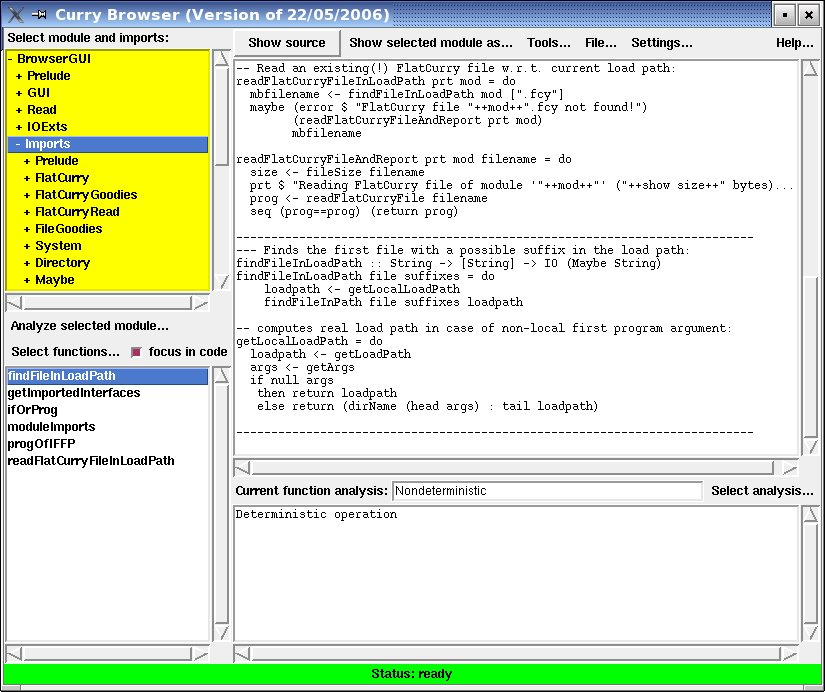
\includegraphics[scale=0.7]{currybrowser.jpg}
\end{center}
\caption{Snapshot of the main window of CurryBrowser\label{fig-currybrowser}}
\end{figure}
%
To get an impression of the use of \cb, Figure~\ref{fig-currybrowser}
shows a snapshot of its use on a particular application
(here: the implementation of \cb).
The upper list box in the left column shows the modules and their imports
in order to browse through the modules of an application.
Similarly to directory browsers, the list of imported modules of a module
can be opened or closed by clicking.
After selecting a module in the list of modules, its source code,
interface, or various other formats of the module can be shown
in the main (right) text area. For instance, one can show
pretty-printed versions of the intermediate flat programs (see below)
in order to see how local function definitions are translated by lambda lifting
\cite{Johnsson85}
or pattern matching is translated into case expressions \cite{Hanus97POPL,Wadler87}.
Since Curry is a language with parametric polymorphism and type inference,
programmers often omit the type signatures when defining functions.
Therefore, one can also view (and store) the selected module as source code where
missing type signatures are added.

Below the list box for selecting modules, there is a menu
(``Analyze selected module'') to analyze all functions
of the currently selected module at once. This is useful
to spot some functions of a module that could be problematic
in some application contexts, like functions that are impure (i.e., the result
depends on the evaluation time) or partially defined (i.e.,
not evaluable on all ground terms).
If such an analysis is selected,
the names of all functions are shown in the
lower list box of the left column (the ``function list'')
with prefixes indicating the properties of the individual functions.

The function list box can be also filled with functions
via the menu ``Select functions''. For instance, all functions
or only the exported functions defined in the currently selected
module can be shown there, or all functions from different modules
that are directly or indirectly called from
a currently selected function.
This list box is central to focus on a function in the
source code of some module or to analyze some function,
i.e., showing their properties. In order to focus on a function,
it is sufficient to check the ``focus on code'' button.
To analyze an individually selected function, one can
select an analysis from the list of available program analyses
(through the menu ``Select analysis'').
In this case, the analysis results are either shown
in the text box below the main text area
or visualized by separate tools, e.g., by a graph drawing tool for
visualizing call graphs.
Some analyses are local, i.e., they need only to consider the local definition
of this function (e.g., ``Calls directly,'' ``Overlapping rules,''
``Pattern completeness''),
where other analyses are global, i.e.,
they consider the definitions of all functions directly or indirectly called
by this function (e.g., ``Depends on,'' ``Solution complete,''
``Set-valued'').
%
Finally, there are a few additional tools integrated into \cb,
for instance, to visualize the import relation between all modules
as a dependency graph. These tools are available through the ``Tools'' menu.

More details about the use of \cb and all built-in analyses
are available through the ``Help'' menu of \cb.


\newpage

\section{CurryTest: A Tool for Testing Curry Programs}
\label{sec-currytest}

CurryTest\index{CurryTest}\index{testing programs}\index{program!testing}
is a simple tool in the KiCS2 distribution to write
and run repeatable tests. CurryTest simplifies the task
of writing test cases for a module and executing them.
The tool is easy to use. Assume one has implemented a module \code{MyMod}
and wants to write some test cases to test its functionality,
making regression tests in future versions, etc.
For this purpose, there is a system library \code{Assertion}
(Section~\ref{Library:Assertion}) which
contains the necessary definitions for writing tests.
In particular, it exports an abstract polymorphic type \ccode{Assertion a}
together with the following operations:
\begin{curry}
assertTrue      :: String -> Bool -> Assertion ()
assertEqual     :: String -> a -> a -> Assertion a
assertValues    :: String -> a -> [a] -> Assertion a
assertSolutions :: String -> (a->Success) -> [a] -> Assertion a
assertIO        :: String -> IO a -> a -> Assertion a
assertEqualIO   :: String -> IO a -> IO a -> Assertion a
\end{curry}
The expression \ccode{assertTrue $s$ $b$}
is an assertion (named $s$) that the expression $b$ has the value \code{True}.
Similarly, the expression \ccode{assertEqual $s$ $e_1$ $e_2$}
asserts that the expressions $e_1$ and $e_2$
must be equal (i.e., \code{$e_1$==$e_2$} must hold),
the expression \ccode{assertValues $s$ $e$ $vs$} asserts
that $vs$ is the multiset of all values of $e$,
and the expression \ccode{assertSolutions $s$ $c$ $vs$} asserts
that the constraint abstraction $c$ has the multiset of solutions $vs$.
Furthermore, the expression \ccode{assertIO $s$ $a$ $v$}
asserts that the I/O action $a$ yields the value $v$ whenever it is
executed, and
the expression \ccode{assertEqualIO $s$ $a_1$ $a_2$}
asserts that the I/O actions $a_1$ and $a_2$ yields equal values.
The name $s$ provided as a first argument in each assertion
is used in the protocol produced by the test tool.

One can define a test program by importing the module
to be tested together with the module \code{Assertion} and defining
top-level functions of type \code{Assertion} in this module
(which must also be exported).
As an example, consider the following program
that can be used to test some list processing functions:
\begin{curry}
import List
import Assertion

test1 = assertEqual     "++"     ([1,2]++[3,4]) [1,2,3,4]

test2 = assertTrue      "all"    (all (<5) [1,2,3,4])

test3 = assertSolutions "prefix" (\x -> let y free in  x++y =:= [1,2])
                                 [[],[1],[1,2]]

\end{curry}
For instance, \code{test1} asserts that the result of evaluating the
expression \code{([1,2]++[3,4])} is equal to \code{[1,2,3,4]}.

We can execute a test suite by the command\pindex{currytest}
\begin{curry}
currytest testList
\end{curry}
(\code{currytest} is a program stored in \code{$kics2home$/bin}
where $kics2home$ is the installation directory of KiCS2;
see Section~\ref{sec-install}).
In our example, \ccode{testList.curry} is the program containing the
definition of all assertions. This has the effect
that all exported top-level functions
of type \code{Assertion} are tested (i.e., the corresponding
assertions are checked) and the results
(\ccode{OK} or failure) are reported together with the name of each assertion.
%If failures occur, the complete test results are also
%written into a file named \ccode{testList.testlog}.''
For our example above, we obtain the following successful protocol:
\begin{curry}
============================================================
Testing module "testList"...
OK: ++
OK: all
OK: prefix
All tests successfully passed.
============================================================
\end{curry}
There is also a graphical interface that summarizes the results
more nicely.
In order to start this interface, one has to add the parameter
\ccode{--window} (or \ccode{-w}), e.g., executing a test suite by
\begin{curry}
currytest --window testList
\end{curry}
or
\begin{curry}
currytest -w testList
\end{curry}
A snapshot of the interface is shown in Figure~\ref{fig-currytest}.

\begin{figure}%[t]
\begin{center}
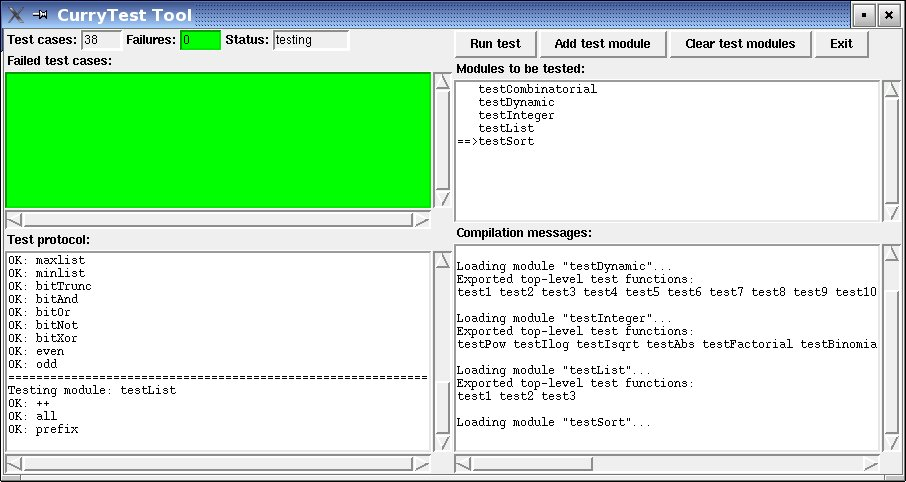
\includegraphics[scale=0.7]{currytest.jpg}
\end{center}
\caption{Snapshot of CurryTest's graphical interface\label{fig-currytest}}
\end{figure}


\newpage

\section{ERD2Curry: A Tool to Generate Programs from ER Specifications}
\label{sec-erd2curry}

ERD2Curry\index{ERD2Curry}\index{database programming}
is a tool to generate Curry code to access and manipulate data
persistently stored from
entity relationship diagrams.\index{entity relationship diagrams}
The idea of this tool is described in detail in
\cite{BrasselHanusMueller08PADL}.
Thus, we describe only the basic steps to use this tool
in the following.

If one creates an entity relationship diagram (ERD)
with the Umbrello UML Modeller, one has to store its
XML description in XMI format (as offered by Umbrello)
in a file, e.g., \ccode{myerd.xmi}.
This description can be compiled into a Curry program by the
command\pindex{erd2curry}
\begin{curry}
erd2curry myerd.xmi
\end{curry}
(\code{erd2curry} is a program stored in \code{$kics2home$/bin}
where $kics2home$ is the installation directory of KiCS2;
see Section~\ref{sec-install}).
If \code{MyData} is the name of the ERD, the Curry program file
\ccode{MyData.curry} is generated containing all the necessary
database access code as described in \cite{BrasselHanusMueller08PADL}.

If one does not want to use the Umbrello UML Modeller,
one can also create a textual description of the ERD
as a Curry term of type \code{ERD}
(w.r.t.\ the type definition given in module
\code{$kics2home$/tools/erd2curry/ERD.curry})
and store it in some file, e.g., \ccode{myerd.term}.
This description can be compiled into a Curry program by the
command\pindex{erd2curry}
\begin{curry}
erd2curry -t myerd.term
\end{curry}
%
There is also the possibility to visualize an ERD term
as a graph with the graph visualization program \code{dotty}
(for this purpose, it might be necessary to adapt the definition
of \code{dotviewcommand} in your \ccode{.kics2rc} file,
see Section~\ref{sec-customization},
according to your local environment).
This can be done by the command
\begin{curry}
erd2curry -v myerd.term
\end{curry}

\paragraph{Inclusion in the Curry application:}
To compile the generated database code, either
include the directory \code{$kics2home$/tools/erd2curry}
into your Curry load path
(e.g., by setting  the environment variable
\ccode{CURRYPATH}\pindex{CURRYPATH}, see also Section~\ref{sec-modules})
or copy the file
\code{$kics2home$/tools/erd2curry/ERDGeneric.curry}
into the directory of the generated database code.


\newpage

\section{Technical Problems}

One can implement distributed systems with KiCS2
by the use of the library \code{NamedSocket} (Section~\ref{Library:NamedSocket})
that supports a socket communication with symbolic names
rather than natural numbers.
For instance, this library is the basis of programming
dynamic web pages with the libraries
\code{HTML} (Section~\ref{Library:HTML})
or \code{WUI} (Section~\ref{Library:WUI}).
However, it might be possible that some technical problems
arise due to the use of named sockets.
Therefore, this section gives some information
about the technical requirements of KiCS2 and how to solve
problems due to these requirements.

There is one fixed port that is used by the implementation of KiCS2:
\begin{description}
\item[Port 8767:] This port is used by the
{\bf Curry Port Name Server} (CPNS) to implement symbolic names for
named sockets in Curry.
If some other process uses this port on the machine,
the distribution facilities defined in the module \code{NamedSocket}
cannot be used.
\end{description}
If these features do not work, you can try to find out
whether this port is in use by the shell command
\ccode{netstat -a | fgrep 8767} (or similar).

The CPNS is implemented as a demon listening on its port 8767
in order to serve requests about registering a new symbolic
name for a named socket or asking the physical port number
of an registered named socket. The demon will be automatically started for
the first time on a machine when a user runs a program
using named sockets.
It can also be manually started and terminated by the
scripts \code{$kics2home$/cpns/start} and
\code{$kics2home$/cpns/stop}.
If the demon is already running, the command \code{$kics2home$/cpns/start}
does nothing (so it can be always executed
before invoking a Curry program using named sockets).

If you detect any further technical problem,
please write to
\begin{center}
\code{mh@informatik.uni-kiel.de}
\end{center}

\newpage

\addcontentsline{toc}{section}{Bibliography}
\bibliography{mh}
\bibliographystyle{plain}

\newpage
\appendix

\section{Libraries of the KiCS2 Distribution}
\label{sec:libraries}

{\setlength{\parindent}{0.0cm}

The KiCS2 distribution comes with an extensive collection
of libraries for application programming.
The libraries for meta-programming by representing
Curry programs as datatypes in Curry are described
in the following subsection in more detail.
The complete set of libraries with all exported types and functions
are described in the further subsections.
For a more detailed online documentation of all libraries of KiCS2,
see \url{http://www-ps.informatik.uni-kiel.de/kics2/lib/index.html}.


\subsection{AbstractCurry and FlatCurry: Meta-Programming in Curry}
\label{sec-flatcurry}

\index{AbstractCurry}
\index{FlatCurry}
To support meta-programming, i.e., the manipulation of Curry programs
in Curry, there are system modules
\code{FlatCurry} (Section~\ref{Library:FlatCurry})
and \code{AbstractCurry} (Section~\ref{Library:AbstractCurry}),
stored in the directory \ccode{$kics2home$/lib/meta},
which define datatypes for the representation
of Curry programs.
\code{AbstractCurry} is a more direct representation of a Curry program,
whereas \code{FlatCurry} is a simplified representation
where local function definitions are replaced by global definitions
(i.e., lambda lifting has been performed) and pattern matching
is translated into explicit case/or expressions.
Thus, \code{FlatCurry} can be used for more back-end oriented
program manipulations (or, for writing new back ends for Curry),
whereas \code{AbstractCurry} is intended for manipulations of
programs that are more oriented towards the source program.

Both modules contain predefined I/O actions to read programs
in the \code{AbstractCurry} (\code{readCurry}\pindex{readCurry})
or \code{FlatCurry}
(\code{readFlatCurry}\pindex{readFlatCurry}) format.
These actions parse the corresponding source program and return
a data term representing this program (according to the definitions
in the modules \code{AbstractCurry} and \code{FlatCurry}).

Since all datatypes are explained in detail in these modules,
we refer to the online documentation\footnote{%
\url{http://www-ps.informatik.uni-kiel.de/kics2/lib/CDOC/FlatCurry.html} and
\url{http://www-ps.informatik.uni-kiel.de/kics2/lib/CDOC/AbstractCurry.html}}
of these modules.

As an example, consider a program file \ccode{test.curry}
containing the following two lines:
\begin{curry}
rev []     = []
rev (x:xs) = (rev xs) ++ [x]
\end{curry}
Then the I/O action \code{(FlatCurry.readFlatCurry "test")} returns the
following term:
\begin{curry}
 (Prog "test"
  ["Prelude"]
  []
  [Func ("test","rev") 1 Public
        (FuncType (TCons ("Prelude","[]") [(TVar 0)])
                  (TCons ("Prelude","[]") [(TVar 0)]))
        (Rule [0]
           (Case Flex (Var 1)
              [Branch (Pattern ("Prelude","[]") [])
                  (Comb ConsCall ("Prelude","[]") []),
               Branch (Pattern ("Prelude",":") [2,3])
                  (Comb FuncCall ("Prelude","++")
                        [Comb FuncCall ("test","rev") [Var 3],
                         Comb ConsCall ("Prelude",":")
                              [Var 2,Comb ConsCall ("Prelude","[]") []]
                        ])
              ]))]
  []
 )
\end{curry}


%%%%%%%%%%%%%%%%%%%%%%%%%%%%%%%%%%%%%%%%%%%%%%%%%%%%%%%%%%%%%%%%%%%%%%%%%
% Definitions in order to LaTeX documents generated by "currydoc --tex"
%%%%%%%%%%%%%%%%%%%%%%%%%%%%%%%%%%%%%%%%%%%%%%%%%%%%%%%%%%%%%%%%%%%%%%%%%

\newcommand{\currymodule}[1]{\subsubsection{Library #1}\label{Library:#1}}
\newcommand{\currytypesstart}{\subsubsection*{Exported types:}}
\newcommand{\currytypesstop}{}
\newcommand{\currytypesynstart}[2]{{\tt type #2}\pindex{#1} \begin{quote}}
\newcommand{\currytypesynstop}{\end{quote}}
\newcommand{\currydatastart}[1]{{\tt data #1}\pindex{#1} \begin{quote}}
\newcommand{\currydatacons}{\end{quote}%
\begin{itemize}\item[] \hspace{-4ex}\emph{Exported constructors:}}
\newcommand{\currydatastop}{\end{itemize}}
\newcommand{\curryconsstart}[2]{\item {\tt #1~::~#2}\par}
\newcommand{\curryfuncstart}{\subsubsection*{Exported functions:}}
\newcommand{\curryfuncstop}{}
\newcommand{\curryfunctionstart}[2]{#2\pindex{#1}\begin{quote}}
\newcommand{\curryfunctionstop}{\end{quote}}
\newcommand{\curryfuncsig}[2]{{\tt #1~::~#2}}


\subsection{General Libraries}

\input{lib/AllSolutions}
\input{lib/Assertion}
\input{lib/Char}
\input{lib/Combinatorial}
\input{lib/Constraint}
\input{lib/CSV}
\input{lib/Directory}
\input{lib/FileGoodies}
\input{lib/Float}
\input{lib/Global}
\input{lib/GUI}
\input{lib/Integer}
\input{lib/IO}
\input{lib/IOExts}
\input{lib/JavaScript}
\input{lib/KeyDatabaseSQLite}
\input{lib/List}
\input{lib/Maybe}
\input{lib/NamedSocket}
\input{lib/Parser}
\input{lib/Pretty}
\input{lib/Profile}
\input{lib/PropertyFile}
\input{lib/Read}
\input{lib/ReadNumeric}
\input{lib/ReadShowTerm}
\input{lib/SetFunctions}
\input{lib/SearchTree}
\input{lib/Socket}
\input{lib/System}
\input{lib/Time}
\input{lib/Unsafe}


\subsection{Data Structures and Algorithms}

\input{lib/Array}
\input{lib/Dequeue}
\input{lib/FiniteMap}
\input{lib/GraphInductive}
\input{lib/Random}
\input{lib/RedBlackTree}
\input{lib/SetRBT}
\input{lib/Sort}
\input{lib/TableRBT}
\input{lib/Traversal}

\subsection{Libraries for Web Applications}

\input{lib/CategorizedHtmlList}
\input{lib/HTML}
\input{lib/HtmlParser}
\input{lib/Mail}
\input{lib/Markdown}
\input{lib/WUI}
\input{lib/URL}
\input{lib/XML}
\input{lib/XmlConv}

\subsection{Libraries for Meta-Programming}

\input{lib/AbstractCurry}
\input{lib/AbstractCurryPrinter}
\input{lib/CompactFlatCurry}
\input{lib/CurryStringClassifier}
\input{lib/FlatCurry}
\input{lib/FlatCurryGoodies}
\input{lib/FlatCurryRead}
\input{lib/FlatCurryShow}
\input{lib/FlatCurryXML}
\input{lib/FlexRigid}
\input{lib/PrettyAbstract}

} % end setlength parindent

\newpage

\input{markdown_syntax}

\newpage

%%%%%%%%%%%%%%%%%%%%%%%%%%%%%%%%%%%%%%%%%%%%%%%%%%%%%%%%%%%%%%%%%%%%%%%
\section{Auxiliary Files}
\label{sec-auxfiles}

During the translation and execution of a Curry program with KiCS2,
various intermediate representations of the source program are created
and stored in different files which are shortly explained in this section.
In general, it is not necessary to know about
these auxiliary files because they are automatically generated
and updated. You should only remember the command for deleting
all auxiliary files (\ccode{cleancurry}, see Section~\ref{sec-general})
to clean up your directories.

The various components of KiCS2 create the following auxiliary files.
\begin{description}
\item[\code{prog.fcy}:] This file contains the Curry program
in the so-called ``FlatCurry'' representation where all functions are global
(i.e., lambda lifting has been performed) and pattern matching
is translated into explicit case/or expressions
(compare Appendix~\ref{sec-flatcurry}).
This representation might be useful for other back ends and
compilers for Curry and is the basis doing meta-programming in Curry.
This file is implicitly
generated when a program is compiled with KiCS2.
The FlatCurry representation of a Curry program is usually
generated by the front-end after parsing, type checking and eliminating
local declarations.
If $dir$ is the directory where the Curry program is stored,
the corresponding FlatCurry program is stored in the directory
\ccode{$dir$/.curry}.

\item[\code{prog.fint}:] This file contains the interface
of the program in the so-called ``FlatCurry'' representation,
i.e., it is similar to \code{prog.fcy} but contains only exported
entities and the bodies of all functions omitted (i.e., ``external'').
This representation is useful for providing a fast access
to module interfaces.
This file is implicitly generated when a program is compiled with KiCS2
and stored in the same directory as \code{prog.fcy}.

\item[\code{Curry_prog.nda}:] This file contains some information about
the determinism behavior of operations that is used by the
KiCS2 compiler (see \cite{BrasselHanusPeemoellerReck11}
for more details about the use of this information).
If $dir$ is the directory where the Curry program is stored,
the corresponding Haskell program is stored in the directory
\ccode{$dir$/.curry/.kics2}.

\item[\code{Curry_prog.info}:] This file contains some
information about the top-level functions of module \code{prog}
that are used by the interactive environment,
like determinism behavior or IO status.
This file is stored in the same directory as \code{Curry_prog.nda}.

\item[\code{Curry_prog.hs}:] This file contains a Haskell program
as the result of translating the Curry program with the
KiCS2 compiler.
This file is stored in the same directory as \code{Curry_prog.nda}.

\item[\code{Curry_prog.o}:] This file contains the object code
of the Haskell program \code{Curry_prog.hs} when the latter program is
compiled in order to execute it.
This file is stored in the same directory as \code{Curry_prog.hs}.

\item[\code{Curry_prog.hi}:] This file contains the interface
of the Haskell program \code{Curry_prog.hs} when the latter program is
compiled in order to execute it.
This file is stored in the same directory as \code{Curry_prog.hs}.

\item[\code{prog}:] This file contains the executable
after compiling and saving a program with KiCS2
(see command \ccode{:save} in Section~\ref{sec:kics2-commands}).

\end{description}


\newpage

%%%%%%%%%%%%%%%%%%%%%%%%%%%%%%%%%%%%%%%%%%%%%%%%%%%%%%%%%%%%%%%%%%%%%%%
\section{External Operations}
\label{sec:external-operations}

\index{operation!external}\index{external operation}
Currently, KiCS2 has no general interface to external operations,
i.e., operations whose semantics is not defined by program rules
in a Curry program but by some code written in another programming
language.
Thus, if an external operation should be added
to the system, this operation must be declared as \code{external}
in the Curry source code
and an implementation for this external operation
must be provided for the run-time system.
An external operation is defined as follows in the Curry source code:
\begin{enumerate}
\item
Add a type declaration for the external operation somewhere
in a module defining this operation (usually, the prelude
or some system module).
\item
For external operations it is not allowed to define any
rule since their semantics is determined by an external implementation.
Instead of the defining rules, you have to write
\begin{curry}
f external
\end{curry}
below the type declaration for the external operation \code{f}.
\end{enumerate}
Furthermore, an implementation of the external operation
must be provided in the target language of the KiCS2 compiler,
i.e., in Haskell, and inserted in the compiled code.
In order to simplify this task, KiCS2 follows some code
conventions that are described in the following.

Assume you want to implement your own concatenation
for strings in a module \code{String}.
The name and type of this string concatenation should be
\begin{curry}
sconc :: String -> String -> String
\end{curry}
Since the primitive Haskell implementation of this operation
does not now anything about the operational mechanism of Curry
(e.g., needed narrowing, non-deterministic rewriting),
the arguments need to be completely evaluated before
the primitive implementation is called.
This can be easily obtained by the prelude operation \code{(\$\#\#)}
that applies an operation to the \emph{normal form} of the given
argument, i.e., this operation evaluates the argument
to its normal form before applying the operation to it.\footnote{%
There is also a similar prelude operation \code{(\$\#)}
which evaluates the argument only to head-normal form.
This is a bit more efficient and can be used for unstructured
types like \code{Bool}.}
Thus, we define \code{sconc} by
\begin{curry}
sconc :: String -> String -> String
sconc s1 s2 = (prim_sconc $\$$## s1) $\$$## s2

prim_sconc :: String -> String -> String
prim_sconc external
\end{curry}
so that it is ensured that the external operation \code{prim_sconc}
is always called with complete evaluated arguments.

In order to define the Haskell code implementing \code{prim_sconc},
one has to satisfy the naming conventions of KiCS2.
The KiCS2 compiler generates the following code for the
external operation \code{prim_sconc} (note that the generated
Haskell code for the module \code{String} is stored in the file
\code{.curry/kics2/Curry_String.hs}):
\begin{curry}
d_C_prim_sconc :: Curry_Prelude.OP_List Curry_Prelude.C_Char
               -> Curry_Prelude.OP_List Curry_Prelude.C_Char
               -> ConstStore
               -> Curry_Prelude.OP_List Curry_Prelude.C_Char
d_C_prim_sconc x1 x2 x3500 = external_d_C_prim_sconc x1 x2 x3500
\end{curry}
The type constructors \code{OP_List} and \code{C_Char}
of the prelude \code{Curry_Prelude}\footnote{Note that all
translated Curry modules are imported in the Haskell code fully qualified
in order to avoid name conflicts.}
correspond to the Curry type constructors for lists and characters.
The Haskell operation \code{external_d_C_prim_sconc}
is the external operation to be implemented in Haskell by the programmer.
The additional argument of type \code{ConstStore}
represents the current set of constraints when this
operation is called. This argument is intended to provide
a more efficient access to binding constraints and can be
ignored in standard operations.

If \code{String.curry} contains the code
of the Curry function \code{sconc} described above,
the Haskell code implementing the external operations
occurring in the module \code{String} must be in the
file \code{External_String.hs} which is located in the same
directory as the file \code{String.curry}.
The KiCS2 compiler appends the code contained in
\code{External_String.hs} to the generated code
stored in the file \code{.curry/kics2/Curry_String.hs}.\footnote{%
If the file \code{External_String.hs} contains also
some import declarations at the beginning, these import declarations
are put after the generated import declarations.}

In order to complete our example, we have to write into the
file \code{External_String.hs} a definition of the Haskell function
\code{external_d_C_prim_sconc}.
Thus, we start with the following definitions:
\begin{curry}
import qualified Curry_Prelude as CP

external_d_C_prim_sconc :: CP.OP_List CP.C_Char -> CP.OP_List CP.C_Char
                        -> ConstStore -> CP.OP_List CP.C_Char
\end{curry}
First, we import the standard prelude with the name \code{CP}
in order to shorten the writing of type declarations.
In order to write the final code of this operation,
we have to convert the Curry-related types
(like \code{C_Char}) into the corresponding Haskell types (like \code{Char}).
Note that the Curry-related types contain information about
non-deterministic or constrained values
(see \cite{BrasselHanusPeemoellerReck11,BrasselHanusPeemoellerReck11WLP})
that are meaningless in Haskell.
To solve this conversion problem, the implementation of KiCS2
provides a family of operations to perform these conversions
for the predefined types occurring in the standard prelude.
For instance, \code{fromCurry} converts a Curry type into the
corresponding Haskell type, and \code{toCurry} converts
the Haskell type into the corresponding Curry type.
Thus, we complete our example with the definition
(note that we simply ignore the final argument representing the
constraint store)
\begin{curry}
external_d_C_prim_sconc s1 s2 _ =
  toCurry ((fromCurry s1 ++ fromCurry s2) :: String)
\end{curry}
Here, we use Haskell's concatenation operation \ccode{++}
to concatenate the string arguments.
The type annotation \ccode{:: String} is necessary
because \ccode{++} is a polymorphic function
so that the type inference system of Haskell
has problems to determine the right instance of the conversion
function.

The conversion between Curry types and Haskell types,
i.e., the family of conversion operation \code{fromCurry}
and \code{toCurry}, is defined in the KiCS2 implementation
for all standard data types.
In particular, it is also defined on function types so that one can
easily implement external Curry I/O actions by using
Haskell I/O actions.
For instance, if we want to implement
an external operation to print some string as an output line,
we start by declaring the external operations in the Curry module \code{String}:
\begin{curry}
printString :: String -> IO ()
printString s = prim_printString $\$$## s

prim_printString :: String -> IO ()
prim_printString external
\end{curry}
Next we add the corresponding implementation in the file
\code{External_String.hs} (where \code{C_IO} and \code{OP_Unit} are the names
of the Haskell representation of the Curry type constructor \code{IO}
and the Curry data type \ccode{()}, respectively):
\begin{curry}
external_d_C_prim_printString :: CP.OP_List CP.C_Char -> ConstStore
                              -> CP.C_IO CP.OP_Unit
external_d_C_prim_printString s _ = toCurry putStrLn s
\end{curry}
Here, Haskell's I/O action \code{putStrLn} of type \ccode{String -> IO ()}
is transformed into a Curry I/O action \ccode{toCurry putStrLn}
which has the type
\begin{curry}
CP.OP_List CP.C_Char -> CP.C_IO CP.OP_Unit
\end{curry}
When we compile the Curry module \code{String},
KiCS2 combines these definitions in the target program so that
we can immediately use the externally defined operation
\code{printString} in Curry programs.

As we have seen, KiCS2 transforms a name like
\code{primOP} of an external operation into the name
\code{external_d_C_primOP} for the Haskell operation
to be implemented, i.e., only a specific prefix is added.
However, this is only valid if no special characters occur
in the Curry names.
Otherwise (in order to generate a correct Haskell program),
special characters are translated into specific
names prefixed by \ccode{OP_}. For instance,
if we declare the external operation
\begin{curry}
(<&>) :: Int -> Int -> Int
(<&>) external
\end{curry}
the generated Haskell module contains the code
\begin{curry}
d_OP_lt_ampersand_gt :: Curry_Prelude.C_Int -> Curry_Prelude.C_Int
                     -> ConstStore -> Curry_Prelude.C_Int
d_OP_lt_ampersand_gt x1 x2 x3500 = external_d_OP_lt_ampersand_gt x1 x2 x3500
\end{curry}
so that one has to implement the operation
\code{external_d_OP_lt_ampersand_gt} in Haskell.
If in doubt, one should look into the generated Haskell code
about the names and types of the operations to be implemented.

Finally, note that this method to connect functions implemented in Haskell
to Curry programs provides the opportunity to connect
also operations written in other programming languages
to Curry via Haskell's foreign function interface.


\newpage
\addcontentsline{toc}{section}{Index}
\printindex


\end{document}

% LocalWords:  KiCS
